\subsection{Boundary Extraction}

Vi kan finde kanten ved først at bruge erosion. Herefter trækker vi så det eroderede billede fra originalen, som vist på Figur~\ref{fig:boundary-extraction-by-erosion}.

\begin{figure}[H]
	\centering
	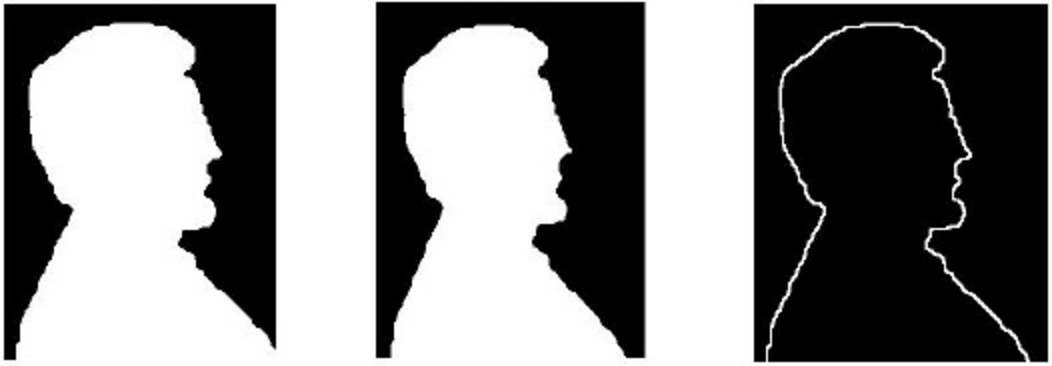
\includegraphics[width=0.9\linewidth]{figs/spm03/boundary-extraction-by-erosion}
	\caption{Fra venstre: Original, efter erosion og til sidst originalen fratrukket erosionen.}
	\label{fig:boundary-extraction-by-erosion}
\end{figure}

Udtrykket for denne operation er vist på Figur~\ref{fig:edgedetektioneq}. 

\begin{figure}[H]
	\centering
	
\includegraphics[width=0.55\linewidth]{figs/spm03/edgedetektioneq}
	\caption{Ligning for boundary extraction ved erosion.}
	\label{fig:edgedetektioneq}
\end{figure}
